\documentclass[a4paper,11pt]{article}
\usepackage[utf8]{inputenc}
\usepackage{amsmath,amssymb,amsfonts}
\usepackage{amsthm}
\usepackage[makeroom]{cancel}
\usepackage{graphicx}
\usepackage{caption}{\tiny }
\renewcommand*\contentsname{İçindekiler}
\renewcommand\refname{}
\renewcommand*\contentsname{}
\usepackage[affil-it]{authblk}
\usepackage[colorlinks = true,
            linkcolor =  black,
            urlcolor  = blue,
            citecolor = blue,
            anchorcolor = blue]{hyperref}

\newcommand{\MYhref}[3][blue]{\href{#2}{\color{#1}{#3}}}%




	\title{\textbf{{\Huge Plazma Salınımı}}}
	\author{{{\huge Halil Kolatan}}}
	\affil{{\large Ankara Üniversitesi,\\ Fen Fakültesi,\\ Fizik Bölümü}}
	\date{{\Large 18 Mayıs 2020}}
	\begin{document}
	\maketitle
	
	\tableofcontents
	
	\newpage
	
	\begin{center}
	\section{Plazma}
	\end{center}



Plazma konusunda yapılan çalışmalar ilk olarak, 1920’li yıllarda Lewi Tonks ve Amerikalı kimyacı ve fizikçi olan Irving Langmuir tarafından yapılmıştır. İlk deneyler gaz deşarjları konusunda yapılmıştır[4, 7]. Yüksek akım taşıyabilen vakum tüplerinin oluşturulmasına
duyulan ihtiyaçtan dolayı yapılan çalışmalarda perdeleme etkisi (shielding effect) keşfedilmiştir. Daha sonra 1930’lu yıllarda kontrollü
nükleer füzyon çalışmalarının başlamasıyla plazma çalışmaları hız kazanmıştır [5, 6, 7]. Sözlük anlamı  elektrik yükü yansız (nötr) olan gaz moleküllerinden, pozitif iyonlardan ve negatif elektronlardan oluşan akışkan anlamına gelse de kimya ve fizikte kısaca iyonize olmuş gaz anlamına gelmektedir. Aynı zamanda maddenin dördüncü hali olarak da bilinmektedir. Gaz fazındaki maddenin çok yüksek sıcaklıklara ısıtılmasıyla atomlar iyonlaşarak, elektron ve pozitif iyonlar oluştururlar. Ancak atomlar tamamıyla iyonize olmamakta ve bir kısmı nötr kalmaya devam edebilmektedir. Oluşan bu parçacık bulutu
plazma olarak adlandırılır. Plazma, soğuk ve
sıcak plazma olarak isimlendirilebilmektedir. Soğuk plazmalarda, gaz fazındaki
atomların sadece \%1-10 kısmı iyonize olmakta geri kalan kısmı ise nötr kalmaya devam
etmektedir. Sıcak plazmalarda gaz tamamen iyonize olmaktadır;
ancak her iyonize gaz plazma değildir [7, 9].

\begin{figure}[h]
	\centering
	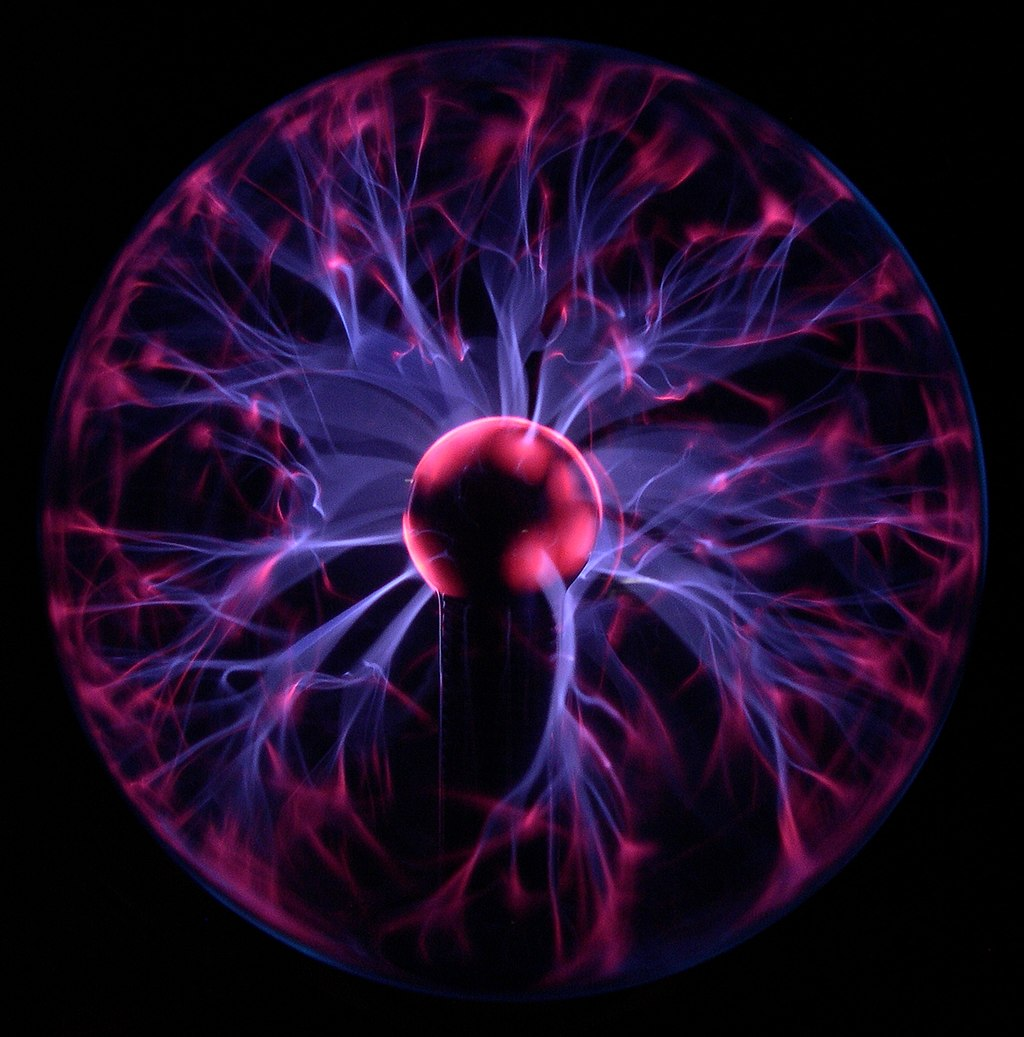
\includegraphics[width=8cm,keepaspectratio=true]{img/lamb.jpg}
	\caption* {\textbf{1.1} Plazma lambası [12].}
\end{figure}

\newpage
	\begin{center}
	\section{Dağınım Bağıntısı}
\end{center}

Bir ortamdaki dağınım bağıntısı dalganın  $\omega$  frekansının  $k$  dalga sayısına nasıl bağlı olduğunu tanımlar [1, 8]. Bir sistem için dağınım bağıntısını tanımlamak,  sistemin dalga davranışını karakterize etmek için uygun bir yoldur. \\

Dalgalarda faz hızı ve grup hızı olmak üzere  iki farklı ilerleme söz konusudur. \\

\subsection{Faz Hızı} Düzlem dalganın belirli bir x noktasını ele alalım. $ kx -\omega t $ faz ifadesi sabit olduğu sürece $\cos(kx -\omega t) $ ifadesi aynı değeri verecek, yani aynı noktanın ilerlemesini takip etmiş olacağız. Bu noktanın hızını hesaplarsak:

\begin{align}
kx -\omega t = sabit
\end{align}
\begin{align}
v_{f} = \dfrac{dx}{dt} = \dfrac{\omega}{t}
\end{align}

faz hızı bulunur  [15]. \\

\subsection{Grup Hızı} Dalga paketi gerçekte genliği modüle eden zarf tarafından oluşturulmuştur. Bu zarfın ilerlemesi paketin ilerlemesi demektir. Bu paket için yine faz bağıntısı yazılırsa:

\begin{align}
\dfrac{\Delta k}{2}x-\dfrac{\Delta \omega}{2}t = sabit
\end{align}
\begin{align}
v_{g} = \dfrac{dx}{dt} = \dfrac{d \omega}{dk}
\end{align}

grup hızı bulunur [15].\\ İkiden fazla frekans bileşeni olan dalgaların ilerleme hızı grup hızıdır. Bilgi grup hızı ile iletilir. Faz hızı ise taşıyıcı dalganın hızıdır. Dağınımsız
dalgalarda faz hızı ve grup hızı aynıdır [14]. 

\newpage
\textbf{Dağınımlı Dalgalar:} $ \dfrac{\omega}{k} \neq sabit $, yani $ \dfrac{\omega}{k} $ dalga boyuna bağlı ise bu dalgalara dağınımlı dalgalar denmektedir. Dağınımlı dalgalarda $ \omega $'nın $ k $'ye göre değişimi incelenir [2].\\

\textbf{Dağınımsız Dalgalar:} $ \dfrac{\omega}{k} = sabit $, dağınım bağıntısını sağlayan dalgalara dağınımsız dalgalar denmektedir  [2]. \\

$ \omega  $ ' nın $ k $ 'ye göre çeşitli dağılımları şekilde  gösterilmiştir [1]. 

\begin{figure}[h]
	\centering
	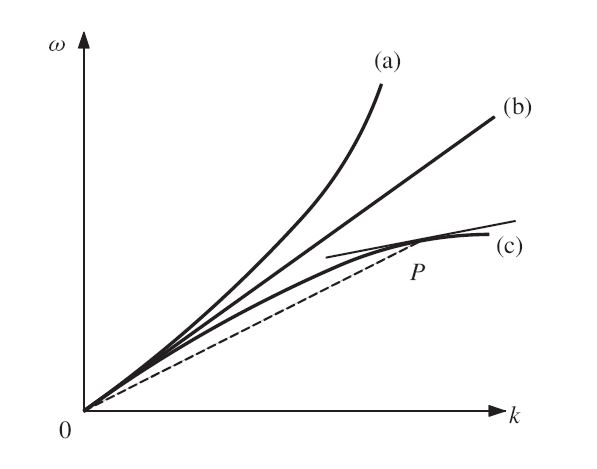
\includegraphics[width=8cm,keepaspectratio=true]{img/Dispersiyon.jpg}
	\caption* {\textbf{1.2} Çeşitli dağınım ilişkileri: $ \omega = \omega (k) $ }
\end{figure}

\begin{itemize}
	\item (a) eğrisi anormal dağılma durumuna karşılık gelir.
    \item (b) eğrisi, dağıtıcı olmayan duruma karşılık gelir.
    \item(c) eğrisi, normal dağılma durumuna karşılık gelir.
\end{itemize}


\newpage 

\begin{center}
	\section{Plazma Salınımı}
\end{center}

Plazma salınımı ya da diğer adıyla Langmuir dalgası, plazma ya da morötesi bölgedeki metal gibi iletken ortamlardaki elektron yoğunluğunda yaşanan salınımlardır. Bu salınımlar, serbest bir elektron gazının dielektrik fonksiyonundaki kararsızlık olarak da tanımlanabilmektedir. Bu salınımların nicemlemeleri sonrasında ortaya çıkan sanki parçacıklar plazmon olarak adlandırılmaktadır [3]. Plazma salınımı, 1920'lerde Irving Langmuir ve Lewi Tonks tarafından keşfedilmiştir [4].\\

\begin{figure}[h]
	\centering
	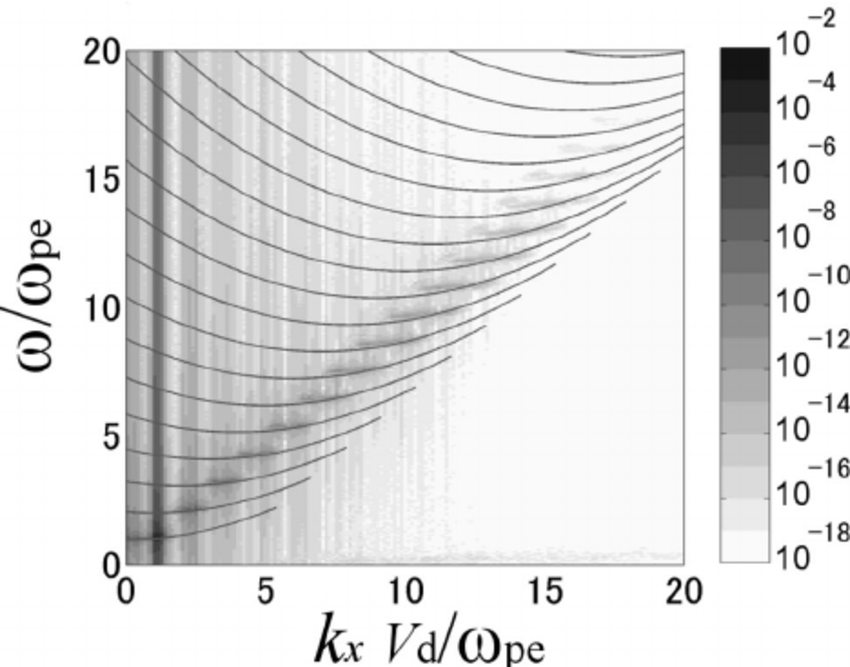
\includegraphics[width=7cm,keepaspectratio=true]{img/Harmonic.jpg}
	\caption* {\textbf{1.3} Harmonik Langmuir dalgaları için simüle edilmiş dağınım bağıntısı [11].}
\end{figure}

Plazma salınımlarının dağınım bağıntısı, çiftlenimli sarkaçlarınkine benzeyen, çok ilginç bir örnektir [2]. \\



Yerkürenin iyonosferinde ki elektromagnetik dalgalar için dağınım bağıntısı:

\begin{align}
\omega^{2}(k) = \omega^{2}_{p} + c^{2} k^{2}, \ \ \omega > \omega_{p}
\end{align}
ve
\begin{align}
\omega^{2}(k) = \omega^{2}_{p} - c^{2} k^{2}, \ \ \omega < \omega_{p}
\end{align}

ile verilir. Burada $ c $ ışık hızıdır, $ \omega_{p} $'de "plazma salınım frekansı" olarak adlandırılan bir büyüklüktür  [2].

\newpage

\begin{align}
\textbf{Plazma Salınım Frekansı:} \quad \omega_{p}^{2} = \dfrac{4 \pi N e^{2}}{m}
\end{align}

Buradaki N elektron yoğunluğunu gösteren sayı, e elektron yükü ve m elektronun kütlesidir. Dağınım bağıntısı $ \omega^{2}(k) = \omega^{2}_{0} + v_{0}^{2} k^{2} $'ye benzeyen bir sistem için mümkün en alçak frekans modunun (k=0), sonsuz dalga boylu bir mod olduğu bilinmektedir. Bu durumda, sarkaçların hepsi aynı faz sabiti ve aynı genlikle salınırlar. $ k=0 $ alındığında plazma frekansı en düşük mod(kip) frekansına eşittir: $\omega_p=\omega_0$. Şimdi bu modu göz önüne alıp ve bunun frekansı olarak plazma salınım frekansını çıkaralım  [2].

Bir nötral plazma, bir miktar iyonlaşmış gaz molekülü ile nötr gaz \\ moleküllerinden oluşmuştur. Bir defa iyonlaşmış her molekül, bir negatif elektronu serbest bırakmış bir pozitif iyondan ibarettir. Yerkürenin iyonosferi birçok iyonlaşmış hava moleküllerinden oluşmuştur. Bir hava molekülünün iyonlaşması güneş ışınlarının morötesi-ışık kuantumlarının soğurulması ile olur. Yerkürenin 200 km'den, 400 km'ye kadar olan yüksekliklerinde iyon yoğunluğu ve serbest-elektron yoğunluğu en büyüktür. Bundan daha yükseklerde elektron ve iyon yoğunluğu azalır çünkü iyonlaşmaya elverişli nötral hava moleküllerinin sayısı azalmıştır. Daha aşağılarda da elektron yoğunluğu azalır çünkü gerekli mor ötesi ışınlar yukarıda soğurulmuştur [2].

\begin{figure}[h]
	\centering
	\includegraphics[width=6cm,keepaspectratio=true]{img/İyonosfer.jpg}
	\caption* {\textbf{1.4} İyonosfer: Güneş ışınları ile iyonize olmuş gaz tabakası [10].}
\end{figure}

\newpage

Plazma nötral olduğundan bir elektrostatik alan kaynağı gibi hareket etmez. Fakat bazen plazmanın herhangi bir bölgesinin yükü hafifçe artabilir. Bu farklılık plazma içerisinde bir elektrik alan oluşturur. Bu elektrik alanın etkisiyle iyonlar bir doğrultuda (alan boyunca), elektronlarda zıt doğrultuda ivmelenirler. Yükler elektrik alanını oluşturan yük fazlalığını ve eksikliğini yok edecek şekilde hareket ederler. Yani Coulomb kuvveti bir geri itme kuvveti oluşturmaktadır.
Elektrik yüklerinin buna bağlı olarak alanın sıfıra düşerek ortadan kaybolduğu süre içinde iyonlar ve elektronlar bir hız kazanmış olurlar. Bu nedenle parçacıkların eylemsizliklerinin yerlerini aşarak yollarına devamlarına ve iyonosferde ilki ile zıt yönde yeni bir yük fazlalığı ve eksikliği doğmasına yol açar. Bu durumda bir defa uyarılınca salınımlarına devam eden bir durum oluşmaktadır  [2].

Eğer sadece yüklerin, bir bölgeden ötekine ileri, geri hareketiyle ilgileniliyorsa, pozitif iyonlar unutulup, elektronların hareketinden doğan yüklü \\ parçacıkların hareketleri ele alınmalıdır. Çünkü elektronlara ve iyonlara etkiyen kuvvet aynı olduğuna göre, elektronların kazandığı ivme kütleler oranı ölçüsünde (bu oran $ 3 \times 10^{4} $ kadardır) çok daha büyük olacaktır  [2]. \\

Plazma iki duvar arasına kapatılmış olsun. 

\begin{figure}[h]
	\centering
	\includegraphics[width=5cm,keepaspectratio=true]{img/plasmanın salınımları.jpg}
	\caption* {\textbf{1.5} Belirli bir bölgeye kapatılmış bir plazmanın salınımları [2].}
\end{figure}
Herhangi bir anda, yük bir duvarda Q kadar artacak, karşı duvarda aynı miktar azalacaktır. Bu farklılık uzayda plazma içinde düzgün bir alan oluşturacaktır  [2].

\begin{align}
\textbf{Alanın Şiddeti:} \quad E_{x} = -4 \pi \dfrac{Q}{A}
\end{align}

Bir elektronun kütlesi m ve yükü $ q $ 'dur. Newton' un ikinci kanunu plazma içindeki her elektron için: 

\begin{align}
m\dfrac{d^{2}x}{dt^{2}}=q E_{x}
\end{align}

şeklindedir. Bir $ cm^{3} $ içerisinde N tane serbest elektron bulunduğunu ve her bir \\ elektronun denge konumundan x kadar yer değiştirdiğini kabul edelim. \\
Bir duvar üzerinde biriken ve karşı duvar üzerinde eksilen net yük:

\begin{align}
Q = N q Ax
\end{align}

ile verilir. Zamana göre iki defa diferensiyeli alınır ve (8) ve (9) yerlerine konulursa:

\begin{align}
\dfrac{d^{2}Q}{dt^{2}} = - \dfrac{4 \pi N q^{2}}{m} Q 
\end{align}


diferensiyel denklemi elde edilir. Bu diferensiyel denklem için aşağıdaki çözümü önerelim:

\begin{align}
Q (t) = Q_{0} \cos (\omega t + \varphi)
\end{align}

\begin{align}
\dfrac{d Q (t)}{dt} = - Q_{0} \sin \omega (\omega t + \varphi)
\end{align}

\begin{align}
\dfrac{d^{2} Q (t)}{dt^{2}} = - Q_{0} \cos \omega^{2} (\omega t + \varphi)
\end{align}

Bu çözüm diferansiyel denklemde yerine koyularak $ \omega^{2} $ bulunur. \\

(11) denklemi, aşağıdaki gibi yazılabilir:

\begin{align*}
\dfrac{d^{2}Q}{dt^{2}} + \dfrac{4 \pi N q^{2}}{m} Q (t)  = 0
\end{align*}

Önerilen çözüm diferensiyel denklemde yerine yazılırsa:

\begin{align}
 - Q_{0} \cos \omega^{2} (\omega t + \varphi) +  \dfrac{4 \pi N q^{2}}{m}  Q_{0} \cos (\omega t + \varphi) = 0
\end{align}
\begin{align}
\cos (\omega t + \varphi) \  Q_{0} \bigg(\dfrac{4 \pi N q^{2}}{m} - \omega^{2}\bigg)  = 0
\end{align}
\begin{align}
 Q_{0} \neq 0,  \ \cos (\omega t + \varphi) \neq 0
\end{align}
\begin{align}
\bigg(\dfrac{4 \pi N q^{2}}{m} - \omega^{2}\bigg) = 0 \Rightarrow \dfrac{4 \pi N q^{2}}{m}  =  \omega^{2}
\end{align}
\begin{align}
\omega^{2} = \dfrac{4 \pi N e^{2}}{m} \equiv \omega_{p} 
\ 
\ \blacksquare
\end{align}


$ \omega_{p}  $'ye plazma salınım frekansı denir.  \\


N, serbest-elektron yoğunluğu yerkürenin iyonosferinde, yükseklikle ve zamanla değişir. İyonların ve elektronların yüksüz moleküller meydana getirecek şekilde birleşimleri güneş battıktan sonra da devam eder, fakat bu arada yeni iyonlar meydana gelmez. Bu yüzden, gece elektron yoğunluğu azalır. Gündüzleri plazma tipik salınım frekansı $ v_{p} = \dfrac{\omega_{p}}{2 \pi} $ 'dir  [2].

\begin{figure}[h]
	\centering
	\includegraphics[width=8cm,keepaspectratio=true]{img/yoğunluk.jpg}
	\caption* {\textbf{1.6} Dünya'nın iyonosferinde ideal elektron yoğunluk dağılımı [13].}
\end{figure}

\newpage
\section{Kaynakça}
\begin{thebibliography}{99}
	
	\bibitem{amano} King, G. (2009).\textit{ Vibrations and Waves}. Wiley. 
	
	\bibitem{mano} Crawford, F. (1969).  \textit{Dalgalar Berkeley Fizik Programı Cilt 2} . Çev., Rauf Nasuhoğlu. Ankara: Güven Yayınları.
	
	\bibitem{mano} Jackson, J. D. (1975).\textit{ Classical Electrodynamics}. New Jersey: Wiley. 
	
	\bibitem{mano} Tonks, L.; Langmuir, I. (1929). \textit{Oscillations in ionized gases}. Phys. Rev., 33, 195-210. doi: 10.1103/PhysRev.33.195.
	
	\bibitem{mano} Cheng, D. (1989).  \textit{Field and Wave Electromagnetics}. Addison-Wesley. 
	
	\bibitem{mano} Chen, F. F. (1974). \textit{Introduction to Plasma Physics}. New York: Plenum Press.
	
	\bibitem{mano} Chen, F. F.; Chang, J. P. (2003).\textit{ Lecture Notes on Principles of Plasma Processing}. New York: Springer. 
	
	\bibitem{mano} Budak, G.; Özdemir, Y. (2014).
    \textit{Titreşimler ve Dalgalar}. Ankara: Nobel Kitap.
    
	\bibitem{mano} Boyd, T. J. M.; Sanderson J. J. (2003). \textit{The Physics of Plasmas}. Cambridge: Cambridge University Press.	
	
	\bibitem{mano} UCAR (2014).  Web sitesi: \MYhref[blue]{https://scied.ucar.edu/ionosphere}{https://scied.ucar.edu/ionosphere}. Erişim tarihi: 17.05.2020.
	
	\bibitem{mano} Umeda, T.; Omura, Y.; Yoon, P.; Gaelzer, R.; Matsumoto, H. (2003). \textit{Harmonic Langmuir waves. III. Vlasov simulation}. Physics of Plasmas, 10, 382-391. \\ doi: 10.1063/1.1537240.
	
	\bibitem{mano} Viatour, L. (2004). Plasma Lamb. Web sitesi:  \MYhref[blue]{https://lucnix.be/}{https://lucnix.be/}. Erişim tarihi: 17.05.2020.
	
	\bibitem{mano} Evans, J. V.; Hagfors, T. (1968). \textit{Radar Astronomy}. McGraw-Hill Education.
	
	\bibitem{mano} Kuru, Ş. (2020).\\ Web Sitesi:\MYhref[blue]{https://acikders.ankara.edu.tr/course/view.php?id=6869}{https://acikders.ankara.edu.tr/course/view.php?id=6869}. Erişim tarihi: 19.05.2020.
	
	\bibitem{mano} Karaoğlu, B. (1998). \textit{Kuantum Mekaniğine Giriş}. Ankara: Güven Yayınları.
	
	
\end{thebibliography}


	
\end{document}          
